\section{Successful heights and concentration across scales}
\label{sec:counting}

We estimate the terms containing at least three core arguments.  Throughout
this section we work on one retained attempt with root $R$, and on one of
the search leaves in the localization.  All the conclusions are uniform
in that leaf.  We use the mode construction, the retained path bounds, and
the notation of Section~\ref{sec:linearization}.  In particular,
$\log D_*\leq\operatorname{poly}(P,k)$, whereas every loss described below
as $P^C$ has an absolute exponent.  The exponent can be increased a finite
number of times without changing this convention.

We first sum the common-height histories and reduce each fixed
configuration to frequency tests with torus amplitude bounds.
A finite sparse-count lemma then controls the tested tuples across
scales.  Finally, interpolation sums the group, amplitude, and
frequency parameters.  The original cell minimum is applied before
subadditivity, keeping each tuple count inside its power; numerical
errors are estimated separately in absolute value.

\subsection{A common successful height}

Fix a term with $m_0\in\{3,4\}$ core roles.  If $m_0=3$, denote the
remaining, side role by $l$.  Fix an actual use $I=I_s$, a group $G$, and
a point $x_*\in I$.  Write $r=|I|$ and $R_s=r^{-1}$.  The choice of $x_*$
is arbitrary; eventually we integrate the resulting estimates over such
points.  All mode lists here are finite.

Sample heights independently and uniformly from the upper height range.
For a fixed tuple of core modes, retain the first sampled height at which
all its roles are good.  A core mode has bad density at most $2\delta_*$
in this range, so the probability of success in one trial is at least
$1-2m_0\delta_*>0$.  Consequently the first-success rule gives an exact
identity in expectation for each pure tuple, and hence for the finite
mode expansion of the form.

Suppose that success occurs at trial $n+1$, with final height $h$.
Assign each of the previous $n$ failed trials to its first failing role,
in the natural order of the roles.  There are at most $m_0^n$ assignments.
For a fixed assignment the conditions in each role form a product mask
on its modes: that role must fail at the trials assigned to it, and must
succeed at the earlier roles' required positions.  Group the selected
modes at the final CURRENT components $\mathcal F_j$.  The coherence of
the upper-height predicates on a minimal CURRENT component implies that
the selected modes are unions of entire core subtotals
$A_{\mathcal D}$ from \eqref{eq:src-26}.  Final success puts all of them
in the unique good predecessor of $\mathcal F_j$.  Let $a_j$ denote the
inherited representative of that predecessor.

Put
\[
 \xi=\frac{\vartheta}{L_{h-\Delta}},\qquad
 \gamma_j^*=\omega_{a_j}(x_*).
\]
A PRE path from a selected mode to its representative gives an integral
vector $n_j$ with $|n_j|_\infty\leq D_*E_{h-\Delta}$ such that its
instantaneous slope at $x_*$ differs from
$\gamma_j^*+n_j\cdot\xi$ by at most $D_*\Xi/r_{v_b}$.
The pre-lag makes the product of this error with $r$ arbitrarily small
at a prescribed inverse power of $D_*$.  The quadratic Taylor error is
equally small: the mode was admitted by $u_b$, and its curvature at its
admission scale was bounded by $D_*$.  The phase constant at $x_*$ can
be absorbed into its coefficient.  Thus the physical selected argument,
up to a uniform error bounded by $D_*^{-150}$ times its absolute
coefficient sum, has the form
\begin{equation*}
 e\big(c_jp^{\rho_j}(y_j)\big)
 e\big(\gamma_j^*(y_j-x_*)\big)
 g_j\big(\xi(y_j-x_*)\big).
 \tag{29}\label{eq:src-29}
\end{equation*}
Here $g_j$ is the true periodic cutoff times a finite trigonometric
polynomial.  Indeed the cutoff is periodic on the $\vartheta$ torus,
and dilation by the integer $L_{h-\Delta}$ makes it periodic on the
$\xi$ torus as well.  We first use this true cutoff when identifying
the progression multiplier, and then use its Fourier truncation.

The cutoff frequencies on this torus have size at most
$B_*L_{h-\Delta}$.  The selected mode frequencies, the cutoff factors,
and the progression multiplier therefore have, in progression
coordinates anchored at any role, their relevant Fourier supports in
\[
 |n|_\infty,|m|_\infty\leq B'_h,
 \qquad B'_h=D_*^5E_{h-\Delta}.
\]
The absolute Fourier costs, apart from the selected absolute mode
coefficient sums themselves, are bounded by fixed powers of $D_*$.
Dilating the torus frequency indices does not change those absolute
coefficient sums.  All precision exponents used here and below are
fixed before the parameter choices; increasing the pre-lag and the
Fourier cutoff by the required fixed powers preserves their polynomial
logarithmic budgets.

If there is a side role, insert in it a fresh cutoff
$\zeta^{\rho_l}$, with $\rho_l$ uniform, divided by its constant
expectation.  That expectation is at least $1/2$.  Set, on $I$,
\[
 S'=\zeta^{\rho_l}e(-c_lp^{\rho_l})S_{\phys}.
\]
Then $\|S'\|_{2,I}\leq\|S\|_{2,I}$.  On the supports of the true
cutoffs the product of all four branch phases is the smooth periodic
progression multiplier constructed in Section~\ref{sec:linearization}.
Write its shifted, truncated version as $R_z(u,v)$, where
$u=\xi(y_{l'}-x_*)$ and $v=\xi t$.  Its supremum is bounded by an
absolute constant, uniformly in every offset and in the anchor $l'$.

\subsection{Torus norms and the frequency tests}

Successful height $h$ supplies a nonexceptional primary.  We can
therefore apply \eqref{eq:src-23} to the pure $\vartheta$ shifts in the
present Fourier boxes.  Let $K_B$ be its rational tiny-frequency
subspace in the horizontal coordinates and set
\[
 \mathbb H=(K_B\cap\Z^{\dim\theta_z})^\perp
 \subseteq\T^{\dim\theta_z}.
\]
The lattice $K_B\cap\Z^{\dim\theta_z}$ is saturated: if a nonzero
integer multiple of an integer vector belongs to it, the vector itself
belongs to the rational subspace $K_B$.  Its annihilator $\mathbb H$
is consequently a connected torus.  For every character difference
in the Fourier ranges under consideration, $r n\cdot\xi$ is tiny when
$n\in K_B$, and is huge otherwise.

Expand the squared modulus of $g_j$ in characters.  Averaging its
restriction to $\xi(I-x_*)$ gives $1$ up to a tiny error for a character
in $K_B$, and a tiny error for every other character, by integration
of an exponential over an interval.  Haar integration on $\mathbb H$
gives exactly $1$ and $0$, respectively.  The difference between these
averages is bounded by $D_*^{-100}$ times the square of the selected
absolute coefficient sum.  The approximation in
\eqref{eq:src-29}, the almost orthogonality of distinct minimal CURRENT
components on $I$, and the floors in \eqref{eq:src-26} thus give
\begin{equation*}
 \begin{split}
 a'_j:=\|g_j\|_{L^2(\mathbb H)}
 &\leq C\left[
 \sum_{\mathcal D\ \mathrm{selected}}
 \left(\|A_{\mathcal D}\|_{2,I}
       +D_*^{-30}
        \sum_{m\ \mathrm{core\ in}\ \mathcal D}|\alpha_m|
 \right)^2\right]^{1/2}.
 \end{split}
 \tag{30}\label{eq:src-30}
\end{equation*}
The augmented norm on the right also bounds the physical norm, so
discarding the private coordinates causes no loss.  The floors absorb
the stated errors even after summing over all components.

We shall use the following Haar estimate.  On $\mathbb H^2$, any pair
of distinct progression coordinates $u+(j-l')v$ and $u+(j'-l')v$ has
independent Haar distribution.  The matrix defining this map has
nonzero integer determinant $j'-j$ and is surjective on a connected
torus; the pushforward of Haar probability is therefore Haar
probability.  Pairwise independence proves the absolute form bound
with two $L^1$ factors and two $L^\infty$ factors.  Multilinear
interpolation among these six bounds gives
\[
 \int_{\mathbb H^2}\prod_{j=0}^3
 |h_j(u+(j-l')v)|\,du\,dv
 \leq\prod_{j=0}^3\|h_j\|_{L^2(\mathbb H)}.
\]
A uniformly bounded multiplier may be inserted at a fixed absolute
cost.  This statement includes the zero-dimensional torus.

Let $U_0=D_*^{250}$.  First suppose that all four roles are core, and
use anchor $l'=0$.  Put
\[
 Q=\sum_j\gamma_j^*,\qquad T=\sum_j j\gamma_j^*.
\]
Seek a pair $n,m$ in the full shift box with
\[
 q'=Q+n\cdot\xi,\qquad t'=T+m\cdot\xi,
 \qquad \max(|q'|,|t'|)\leq U_0R_s.
\]
If such a pair exists, choose one by a fixed rule independent of all
sampling histories and mode masks.  Let $\mu\leq1\leq\nu$ be dyadic
parameters, with fixed endpoint conventions, such that
\begin{equation*}
 \mu\asymp\min\left(1,\min_{0\leq j\leq3}
                   \frac{|t'-jq'|}{R_s}\right),
 \qquad
 \nu\asymp\max\left(1,\frac{|q'|}{R_s},
                           \frac{|t'|}{R_s}\right).
 \tag{31}\label{eq:src-31}
\end{equation*}
We discard a tuple if no reference exists or if the inner minimum in
\eqref{eq:src-31} is smaller than $U_0^{-1}$.  These discards have the
small absolute errors specified below.

Here is the Fourier estimate behind this assertion.  In normalized
anchor coordinates write the kernel as $W_s(h,v)$ and put
\[
 D(u,v)=R_z(u,v)\prod_jg_j(u+jv).
\]
Expanding $D$ samples the Fourier transform of $W_s$ at the frequency
pairs $r(Q+n\cdot\xi,T+m\cdot\xi)$.  Two pairs that are both moderate
must have the same pair of character cosets modulo $K_B$, by the
tiny/huge dichotomy.  Within those cosets their real frequencies differ
from the reference by a tiny quantity, so the sampled Fourier values
may be replaced by the reference value.  Every other coset contributes
only the rapidly decaying Fourier tail.  The sum of the coefficients
in the retained coset pair is
\[
 \int_{\mathbb H^2}D(u,v)e(-n\cdot u-m\cdot v)\,du\,dv,
\]
whose absolute value is at most $C\prod_ja'_j$ by the preceding Haar
estimate.  The four vanishing marginals of the kernel say that its
Fourier transform vanishes on all four lines $t'=jq'$.  Smoothness,
the mean value theorem near those lines, and rapid decay away from
the origin show that its reference value is bounded by
$C_L\mu\nu^{-L}$ for every fixed $L$.  We obtain
$C_L\mu\nu^{-L}\prod_ja'_j$.  If no moderate reference exists, rapid
decay instead gives a negligible contribution.  If the minimum is
less than $U_0^{-1}$, the vanishing-line bound does the same.

Now suppose that there are three core roles and use anchor $l'=l$.
Set
\[
 Q=\sum_{j\ne l}\gamma_j^*,\qquad
 T_l=\sum_{j\ne l}(j-l)\gamma_j^*.
\]
Seek $m$ in the shift box with $|T_l+m\cdot\xi|\leq U_0R_s$ and choose
a reference independently of masks as above.  Write
$\beta=r(T_l+m\cdot\xi)$, and discard when no reference exists or when
$|\beta|<U_0^{-1}$.  In this case set
$\mu\asymp\min(1,|\beta|)$ and
$\nu\asymp\max(1,|\beta|)$.

Fourier integration in the $t$ variable gives a smooth function
$W_\beta(h)$ supported in the normalized interior of the anchor
interval.  Every fixed number of its $h$ derivatives is bounded by
$C_L\mu\nu^{-L}$.  Indeed the anchor marginal vanishes at $\beta=0$,
and integration by parts in $t$ gives decay for large $\beta$.
Only the reference $m$ coset can contribute appreciably.  With
\[
 D(u,v)=R_z(u,v)\prod_{j\ne l}g_j(u+(j-l)v),\qquad
 D_m(u)=\int_{\mathbb H}D(u,v)e(-m\cdot v)\,dv,
\]
duality and the four-factor Haar estimate give
\[
 \|D_m\|_{L^2(\mathbb H)}\leq C\prod_{j\ne l}a'_j.
\]
Collect its horizontal Fourier coefficients by character cosets and
choose one reference $n$ in the box for each coset.  Parseval bounds
the resulting coefficient sequence in $\ell^2$ by the displayed norm.
Different reference frequencies $r n\cdot\xi$ are separated by more
than $1$.  Replacing the other frequencies of the coset by its
reference again costs only a tiny absolute error.

Expand $S'$ in normalized Fourier coefficients on $I$, writing
$\widehat{S'}_I(k')$ for the coefficient of
$e(k'(y-x_*)/r)$, $k'\in\Z$.  The matrix of remaining pairings has
entries bounded, for arbitrarily large fixed $A$, by
\[
 C_{L,A}\mu\nu^{-L}
       (1+|k'+r(Q+n\cdot\xi)|)^{-A}.
\]
In a shell of radius $\Lambda$, the number of nonzero entries in any
row or column is $O(\Lambda)$, since the $k'$ are integers and the
reference real frequencies are $1$-separated.  Schur's inequality,
with $A$ increased to absorb this count, bounds that shell by
$C_L\mu\nu^{-L}\Lambda^{-L}\prod a'_j$ times the $\ell^2$ mass of
$\widehat{S'}_I$ in the corresponding windows.  Averaging the fresh
offset and applying Cauchy--Schwarz proves the bound
\begin{equation*}
 \begin{split}
 C_L\mu\nu^{-L}\prod_{j\ne l}a'_j
       \sum_{\substack{\Lambda=1,2,4,\ldots\\\Lambda\leq U_0}}
             \Lambda^{-L}b_\Lambda,\qquad
 b_\Lambda^2
 =\E_{\rho_l}\!!
 \sum_{\substack{k'\in\Z:\
       |k'+r(Q+n\cdot\xi)|\leq2\Lambda\\
       \text{for some }n\in\Z^{\dim\theta_z},\ |n|_\infty\leq B'_h}}
       |\widehat{S'}_I(k')|^2.
 \end{split}
 \tag{32}\label{eq:src-32}
\end{equation*}
Shells larger than $U_0$ have negligible total contribution.  Notice
that the windows in this definition use the whole Fourier box and
therefore do not depend on the mode masks.  The same fresh offset can
be used for all triples being tested at this cell.

For completeness, all the scalar errors and discarded terms just used
are bounded by
\[
 C D_*^{-100}\prod_{j\ \mathrm{core}}
       \sum_{m\ \mathrm{selected}}|\alpha_m|,
\]
multiplied by the local side size when a side is present.  This follows
term by term from the Fourier tails, the pre-lag, the tiny-frequency
widths, and the smooth kernel estimates.  For the last high-shell
error in \eqref{eq:src-32}, use ordinary $L^2$ pairing or the same
Schur estimate.  These errors do not pay for the number of failure
masks: expand the absolute coefficient sums first, and each pure
tuple has total first-success weight exactly one.  The path count
and coefficient bounds in $D_*$, together with the retained size
caps, make their integrated sum $O(e^{-k}|R|)$.  They will always be
estimated absolutely, before taking a power less than one.

Fix the final height and its component tuple.  If an assignment of
$n$ previous failures assigns $n_j$ of them to role $j$,
\eqref{eq:src-30} and the predicate coherence give
\[
 a'_j\leq C\sigma_{\mathcal F_j},\qquad
 \E(a'_j)^2\leq C(2\delta_*)^{n_j}
                       \sigma_{\mathcal F_j}^2.
\]
To see the second inequality, apply the probability bound to each
selected minimal-component summand of \eqref{eq:src-30}; ignoring
additional success conditions only increases the probability.
H\"older with $m_0$ factors, using the deterministic bound to pass
from second to $m_0$th moments, yields
\[
 \E\prod_j a'_j
 \leq C^{m_0}(2\delta_*)^{n/m_0}
                        \prod_j\sigma_{\mathcal F_j}.
\]
The sum over $m_0^n$ assignments and all $n$ is finite, since the
fixed $\delta_*$ was chosen sufficiently small.  Summing over final
heights, types, and dyadic amplitude bins, we have therefore proved
an absolute cell bound, apart from the errors, by the sum of terms
\begin{equation*}
 C_L\mu\nu^{-L}\Lambda^{-L}
       \left(\prod_{j=0}^3\sigma_j\right)N_s^G.
 \tag{33}\label{eq:src-33}
\end{equation*}
For a core role, $\sigma_j$ is the dyadic bin of the size in
\eqref{eq:src-26}; for a side it is the bin of $b_\Lambda$ in
\eqref{eq:src-32}.  Zero-sized factors have zero contribution.  For
four cores we put $\Lambda=1$.  With all these choices fixed,
$N_s^G$ is the number of core label tuples passing the nonnegligible
tests at $I_s\ni x_*$.  A label tuple is counted at most once at a
given scale.  The useful power estimate will retain this count inside
the power in \eqref{eq:src-33}.

\subsection{A finite sparse-count lemma}

The following finite statement isolates the combinatorial argument.
The fourth role in its three-core case is represented by a square
budget; that role is essential to the proof.

\begin{lemma}[Sparse mass of separated progression tests]
\label{lem:finite-sparse-count}
There are absolute constants $C$ and $C_{\mathrm{res}}$ with the
following property.  There are four roles $0,1,2,3$, of which either
four or exactly three are designated core roles; write $J$ for their
set.  Let $M,L\geq1$, $d\geq0$, $B\geq1$, and
$0<\mu\leq1\leq\nu$.  In each core role $i$ let $\mathcal A_i$ be
a finite set of labels, identified injectively with real numbers,
with $|\mathcal A_i|\leq M$.  Fix $\zeta\in\R^d$.

For finitely many distinct integer indices $s$, let
$R_s=R_0 2^s$ and let $\mathcal E_s\subseteq\prod_{i\in J}\mathcal A_i$
be a set of tuples; put $N_s=|\mathcal E_s|$.  Assume the following.
\begin{enumerate}
\item Two labels in distinct core roles determine at most one full
core tuple among all the $\mathcal E_s$, and the pair has at most
$L$ scale occurrences.
\item If $l$ is a side role, there are $w_s\geq0$ with
$\sum_s w_s\leq M$ such that, at scale $s$, the number of tuples
incident to any fixed core label is at most $w_s$.
\item If distinct labels $a,a'$ in the same core role occur at scales
$s,t$, respectively, then
\[
 |a-a'+n\cdot\zeta|>\Sigma\max(R_s,R_t)
 \qquad(n\in\Z^d,\ |n|_\infty\leq Q).
\]
\item For every triple $T\subseteq J$ of core roles, let $l'$ be the
excluded role and set $\alpha_i=i-l'$ for $i\in T$.  Every tuple at
scale $s$ has, for this triple, a witness $n\in\Z^d$, $|n|_\infty\leq B$,
such that
\[
 \mu R_s\leq
 \left|\sum_{i\in T}\alpha_i a_i+36n\cdot\zeta\right|
 \leq\nu R_s.
\]
\item At every occupied scale $s$,
\[
 |n\cdot\zeta|\notin
 [\mu R_s/1000,1000\nu R_s]
 \qquad(n\in\Z^d,\ |n|_\infty\leq Q).
\]
\end{enumerate}
Suppose that
\[
 Q\geq C_{\mathrm{res}}(d+1)^2B,
 \qquad \Sigma\geq C_{\mathrm{res}}(d+1)^2\nu.
\]
Then, with $\ell=1+\log_2(2+(d+1)^2\nu/\mu)$, one has
\[
 \sum_{s:\ N_s\leq\delta M^2}N_s
 \leq C\ell L^{29}\delta^{1/2080}M^2
 \qquad(0<\delta\leq1).
\]
The constants and exponents are independent of $d$, the real
frequencies, the number of scales, and all label cardinalities.
\end{lemma}

\begin{proof}
We give the cardinality argument on a common fine grid.  This entails
no restriction on the real data.  There are finitely many labels,
scales, and shifts of size at most $Q$.  Approximate their real
coordinates on one grid, taking label and frequency approximants on
a fixed multiple of its step so that the divisions by $1,2,3$ below
remain on the grid.  Separation remains valid with, for example,
$\Sigma/2$; the annular bounds remain valid with $\mu/2$ and $2\nu$;
and the wide pure-shift gap retains the narrower interval
$[\mu R_s/100,100\nu R_s]$ needed after relaxing the parameters.
These assertions follow by choosing the step after all the
finite data, and sufficiently small relative to the least $R_s$.
Round interval widths upward by at most one grid step.  All such
changes cost fixed constants, absorbed in $C_{\mathrm{res}}$ and $C$.
No final estimate depends on the step.  It therefore suffices to
prove the grid version with these harmless fixed margins.  We keep
the original letters for the relaxed parameters.

\paragraph{A graph with many four-step paths.}
We first record the precise graph observation to be used.  Suppose
that a bipartite graph has parts of size at most $M$, at least
$\eta M^2$ edges, and a proper edge coloring with at most $M$ colors,
where $0<\eta\leq1$.  Pad the second part to
$m=\lceil M\rceil\leq2M$ points, choose a uniformly random point in
that part, and let $Y$ be its neighborhood.  Then
\[
 \E|Y|^2\geq(\E|Y|)^2\geq\eta^2M^2/4.
\]
Call an ordered pair in the first part bad if its codegree is less
than $c_0\eta^2M$, with $c_0>0$ a sufficiently small absolute
constant.  Its probability of lying in $Y^2$ is its codegree divided
by $m$.  Summing over the at most $M^2$ ordered pairs gives an expected
number of bad pairs at most $c_0\eta^2M^2$.  It follows, by considering
$|Y|^2-100$ times this number, that some $Y$ has
$|Y|\geq c\eta M$ and fewer than $|Y|^2/100$ bad ordered pairs.
Delete the points with more than $|Y|/4$ bad partners.  Fewer than
$|Y|/25$ points are deleted.  For two retained points there are at
least $c|Y|$ points of $Y$ that are good partners of both.  Each
such midpoint has at least $c_0\eta^2M$ common neighbors with each
endpoint.  Choosing those two neighbors independently shows that
any two retained points have at least
\[
 c\eta^5 M^3
\]
four-step paths between them, allowing repeated vertices.  For fixed
endpoints the ordered four-color tuples of these paths are distinct:
the start vertex and a color determine the next edge uniquely, by
proper coloring, and this reconstructs the whole path successively.

\paragraph{Counting blocks and difference covers.}
Restrict to the scales with $N_s\leq\delta M^2$.  The first hypothesis
gives total mass at most $LM^2$.  Choose parameters
$\delta\leq\alpha/2$ and $0<\kappa<1$, whose values will be fixed at
the end.  Order the retained scales by descending $R_s$, and form
consecutive blocks of mass at most $\alpha M^2$, greedily.  Every
block except possibly the last has mass greater than
$(\alpha-\delta)M^2$.  The number $J_0$ of blocks is therefore at most
$3L/\alpha$.  These are counting blocks, unrelated to the depth
blocks used in the linearization.

Let $R_{\mathfrak b}^+$ be the largest reciprocal scale in a counting
block $\mathfrak b$.  With grid step $h_0$, set
\[
 N_0=\lceil32B\rceil,\qquad
 \epsilon_{\mathfrak b}
 =h_0\left\lceil\frac{16\nu R_{\mathfrak b}^+}{h_0}\right\rceil,
\]
taking $h_0$ small enough that
$\epsilon_{\mathfrak b}\leq17\nu R_{\mathfrak b}^+$ for every block.
For an integer $t\geq1$ define the finite symmetric neighborhood
\[
 U_{\mathfrak b}(t)=
 \{6n\cdot\zeta+u:
       n\in\Z^d,\ |n|_\infty\leq tN_0,
       \ u\in h_0\Z,\ |u|\leq t\epsilon_{\mathfrak b}\}.
\]
These neighborhoods contain zero and satisfy
$U_{\mathfrak b}(t)+U_{\mathfrak b}(t')
 \subseteq U_{\mathfrak b}(t+t')$.

Fix a core role $i$ and a block.  As long as the mass whose $i$-label
is still uncovered exceeds $\kappa M^2$, choose two other core roles
$j,k$.  Project these occurrences to a simple graph of $(i,j)$
pairs, keeping one scale witness in the block for each pair.  There
are at least $(\kappa/L)M^2$ edges.  Color a pair by its $k$-label.
The coloring is proper, because a pair in the roles $(i,k)$ or
$(j,k)$ also determines the entire tuple.  Apply the preceding
observation with $\eta=\kappa/L$ to obtain a subset $B_0$ of role
$i$, of size at least $c\eta M$.

For a four-step path between $a,a'\in B_0$, alternately add and
subtract the four annular relations for the triple $i,j,k$.
The intermediate $i$-label and both $j$-labels cancel.  Division by
$\alpha_i\in\{\pm1,\pm2,\pm3\}$ gives
\[
 a-a'\in q(c_1,c_2,c_3,c_4)+U_{\mathfrak b}(1),
\]
where $q$ depends only on the four colors.  The scalar error is at
most $4\nu R_{\mathfrak b}^+$ before division.  The shift has size
at most $4B$ before division, and $36/\alpha_i$ is an integer
multiple of $6$, which explains the choice of $U_{\mathfrak b}$.

Choose a maximal packing in $B_0-B_0$ whose distinct differences lie
outside $U_{\mathfrak b}(2)$.  Choose one endpoint pair for each
packed difference.  Each has at least $c\eta^5M^3$ ordered
four-color tuples, and two packed differences cannot use the same
tuple, since that would put their difference in
$U_{\mathfrak b}(1)-U_{\mathfrak b}(1)$.  There are at most $M^4$
color tuples in total.  The packing thus has size at most
$C\eta^{-5}M$, and maximality covers $B_0-B_0$ by that many
translates of $U_{\mathfrak b}(2)$.  Remove $B_0$ and repeat.
Each iteration removes at least $c\eta M$ labels, so there are at
most $C\eta^{-1}$ iterations.  We have proved that, except for
$\kappa M^2$ uncovered occurrences in each core role and block,
the incident labels are covered by at most
\[
 K_1=C(L/\kappa)^6
\]
subsets $B$, each of whose difference set is covered by at most
$K_1M$ translates of that block's $U_{\mathfrak b}(2)$.

\paragraph{Nonfuture pairs.}
Discard every occurrence missing an own-block covered label in any
core role.  This loses at most $4J_0\kappa M^2$.  A core role on a
remaining occurrence is called future if its exact label belongs to
a cover subset of that role in a later counting block.  The sets of
nonfuture allowed labels are disjoint over blocks, separately in
each core role: appearance in a later cover would make the earlier
one future.  If $m_i^{\mathfrak b}$ is the number of such labels,
then $\sum_{\mathfrak b}m_i^{\mathfrak b}\leq M$.  The side role is
always nonfuture, and in that role set
$m_l^{\mathfrak b}=\sum_{s\in\mathfrak b}w_s$, which has the same
sum bound.

An occurrence with fewer than three future roles has at least two
nonfuture roles.  Assign one such pair to it.  For a fixed pair the
mass in block $\mathfrak b$ is at most
\[
 \min\big(\alpha M^2,
            Lm_i^{\mathfrak b}m_j^{\mathfrak b}\big).
\]
For two cores this is pair multiplicity; for a core and the side it
is the side incidence budget, with the harmless factor $L\geq1$.
The sum over blocks is at most
\[
 \sqrt{L\alpha}\,M
 \sum_{\mathfrak b}
       \sqrt{m_i^{\mathfrak b}m_j^{\mathfrak b}}
 \leq\sqrt{L\alpha}\,M^2.
\]
There are at most six role pairs.

Every remaining occurrence has three future core roles.  Assign
one such triple and, for each of its labels, one future cover subset
containing it, using fixed rules if there are choices.  The number
of resulting combinations is at most
$4J_0(J_0K_1)^3$.  Fix a combination with mass $\rho M^2>0$.
It consists of a current block, a fixed triple of roles, and subsets
$B_1,B_2,B_3$ in those roles from strictly later blocks.  The indices
$1,2,3$ in the next paragraphs enumerate these roles, and do not
change their progression coefficients $\alpha_i$.

\paragraph{Four ranges with scale margins.}
Set
\[
 \Gamma=C_{\mathrm{gap}}(d+1)^2\nu/\mu,
\]
where $C_{\mathrm{gap}}$ is a sufficiently large absolute constant.
If $\rho\leq C\delta\ell$, retain this bound and do no further work
on the combination.  Otherwise increase the absolute $C$ so that
all the following margins hold.  Cut the ordered mass at its three
quartiles and omit the individual scale bins crossing the cuts.
At most three bins are lost, each of mass at most $\delta M^2$.
Each of the four remaining ordered ranges has mass at least
$\rho M^2/8$, and hence at least $\rho/(8\delta)$ occupied dyadic
bins.  Write $R^\#$ for the largest reciprocal scale of the second
range.

The first range supplies, in each $B_i$, a set $B_{i0}$ of distinct
anchor labels with
\[
 |B_{i0}|\geq c\rho M/L.
\]
Indeed a fixed label is incident to at most $LM$ occurrences, by
pair determination and multiplicity with any other core role.
Each anchor has an occurrence at reciprocal scale at least $R^\#$,
so distinct anchors are separated modulo the reserved shifts by
more than $\Sigma R^\#$.

The last range supplies a set $F$ of distinct actual triples with
\[
 |F|\geq c\rho M^2/L,
\]
choosing one scale witness for each.  A triple has at most $L$
occurrences.  The third range contains at least $\rho/(8\delta)$
occupied dyadic bins.  Thus every second-range reciprocal scale
exceeds every last-range reciprocal scale by a factor at least
$\Gamma$, once $\rho>C\delta\ell$.  Every future block lies below
the entire current block in reciprocal scale, so the same assertion
holds for every future-block scale used by this combination.
Greedily thin the second range so that successive selected scales
have ratio at least $\Gamma$.  Each selection excludes at most
$1+\lceil\log_2\Gamma\rceil\leq C\ell$ occupied bins, and therefore
retains
\[
 q\geq c\rho/(\delta\ell)
\]
scales.  Choose one actual triple $t_v$ at each selected scale $R_v$.
Figure~\ref{fig:counting-blocks} shows the four ranges for this fixed combination.

\begin{figure}[t]
 \centering
 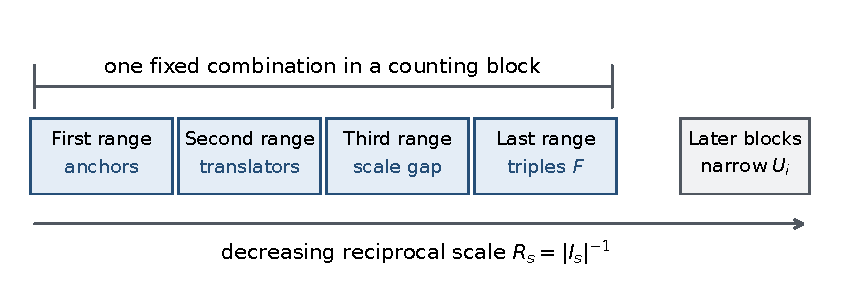
\includegraphics[width=\linewidth]{figures/counting-blocks.pdf}
 \caption{For one fixed choice of a current counting block, three
 core roles, and their future cover subsets, the four ranges shown
 remain after omitting the scale bins crossing the quartile cuts.
 Reciprocal scale decreases from left to right.  The ranges supply
 anchors, separated translators, a scale gap, and the set $F$.
 The selected future subsets lie in later counting blocks and have
 narrower neighborhoods.  These counting blocks are distinct from
 the consecutive $K$-depth blocks in Figure~\ref{fig:depth-blocks}.}
 \label{fig:counting-blocks}
\end{figure}

We will compare the $q|F|$ indexed outputs of the translated sets
$t_v+F$ with a cover of a common slab.  The next two steps build
covers of the future sumsets; the anchors will remove one factor
$M$ from the slab cover.  The scale margins will then show that
no cover box contains two of these outputs.

\paragraph{A small-growth scale without an exponential loss.}
Write $U_i$ and $\epsilon_i$ for the neighborhoods and widths of the
future block associated with $B_i$.  Subdividing each coefficient
interval and the scalar interval gives, for every integer $t\geq1$,
a cover of $U_i(t)$ by at most $(2t+1)^{d+1}$ translates of $U_i(1)$.
Consequently there is an odd integer
\[
 1\leq H_i\leq100(d+1)^2,
 \qquad |U_i(H_i+2)|\leq2|U_i(H_i)|.
\]
Otherwise growth by more than $2$ at each odd step would exceed
the displayed polynomial-in-$t$ bound by the time $t$ is a
sufficiently large absolute multiple of $(d+1)^2$.  The exponential
dependence on $d$ of the preliminary cover is used only for this
choice of $H_i$; it is not paid in the estimates below.

The translates $a+U_i(H_i)$, $a\in B_{i0}$, are disjoint.  An
intersection would put their difference in $U_i(2H_i)$, whose
shift index in the $\zeta$ lattice is $O((d+1)^2B)$ and whose
scalar width is at most $C(d+1)^2\nu R^\#$.  The reserves on
$Q$ and $\Sigma$ exclude this.  With
$Z_i=B_{i0}+U_i(H_i)$, the difference cover for $B_i-B_i$ gives
\[
 \begin{split}
 |Z_i-B_i|
 &\leq K_1M|U_i(H_i+2)|
 \leq2K_1M|U_i(H_i)|\\
 &\leq C(K_1L/\rho)|Z_i|.
 \end{split}
\]

\paragraph{The minimal-growth subset argument.}
Choose a nonempty $X_i\subseteq Z_i$ minimizing
$r_i=|X_i-B_i|/|X_i|$.  Then $r_i\leq CK_1L/\rho$.
We include the iteration argument, in the form used in
\cite{Petridis2012}.  For a finite family of translates
$C_0=\{c_1,\ldots,c_q\}$ let $X_{i,j}$ consist of the points $x\in X_i$
whose translate $x+c_j$ is not in any earlier $X_i+c_v$.
Thus $|X_i+C_0|=\sum_j|X_{i,j}|$.  Every point of
$(X_i\setminus X_{i,j})-B_i+c_j$ already belongs to an earlier
translate of $X_i-B_i$.  The new points contributed at step $j$
are therefore at most
\[
 \begin{split}
 |X_i-B_i|-|(X_i\setminus X_{i,j})-B_i|
 &\leq r_i|X_i|-r_i|X_i\setminus X_{i,j}|\\
 &=r_i|X_{i,j}|,
 \end{split}
\]
by minimality; the empty-complement case is included.  Summing and
then iterating with $C_0=-(m-1)B_i$ proves
\[
 |X_i-mB_i|\leq r_i^m|X_i|\qquad(m\geq1),
\]
where $mB_i$ denotes the $m$-fold sumset.

One anchor translate contains a portion $Y_i$ of $X_i$ of size at
least $|X_i|/M$, since there are at most $M$ anchors.  Its difference
set is contained in $U_i(2H_i)$.  If $\mathcal P$ is a packing of
$mB_i$ with distinct differences outside $U_i(2H_i)$, the translates
$Y_i-p$, $p\in\mathcal P$, are disjoint and belong to $X_i-mB_i$.
Hence
\[
 |\mathcal P|\leq r_i^m M.
\]
Maximal packings give covers by the same neighborhood.  We need
only $m=2,3$.

\paragraph{A slab cover with only two label-count factors.}
Put $r_0=CK_1L/\rho$, enlarging the absolute constant so that
$r_i\leq r_0$ for every role.  Consider the set of outputs in
$2B_1\times2B_2\times2B_3$ satisfying
\[
 \left|\sum_i\alpha_i x_i+36n\cdot\zeta\right|
       \leq2\nu R^\#
 \quad\text{for some }n\in\Z^d,\quad |n|_\infty\leq2B.
\]
Cover the first two sumsets by at most $r_0^2M$ translates each
of $U_i(2H_i)$.  Above a fixed pair of boxes, the possible third
coordinate lies in $2B_3$ intersected with a set of the form
\[
 c+\{n\cdot\zeta:|n|_\infty\leq C(d+1)^2B\}
       +[-C(d+1)^2\nu R^\#,C(d+1)^2\nu R^\#].
\]
Indeed substitute the first two coordinate boxes into the slab
relation and divide by $\alpha_3\in\{\pm1,\pm2,\pm3\}$.
The box shifts are $6n\cdot\zeta$ and the slab shifts are
$36n\cdot\zeta$, so the divided coefficients remain integral.
Their sizes have the stated bound.

Let $\mathcal P$ be a packing in this local third-coordinate set
outside $U_3(2H_3)$.  Then $B_{30}+\mathcal P\subseteq3B_3$ is
still such a packing.  For an equal anchor this is the definition
of $\mathcal P$.  For distinct anchors, a collision would express
their difference, modulo a reserved shift, with absolute value at
most $C(d+1)^2\nu R^\#$, contradicting their separation.  The
global $3B_3$ packing bound gives
\[
 |B_{30}|\,|\mathcal P|\leq r_0^3M,
 \qquad |\mathcal P|\leq Cr_0^3L/\rho.
\]
Covering the local third-coordinate set by a maximal packing shows
that the whole slab is covered by at most
\[
 C r_0^7(L/\rho)M^2
 \leq C K_1^7(L/\rho)^8M^2
\]
translates of $\prod_{i=1}^3U_i(2H_i)$.  The use of all the
separated anchors is what removes a third factor $M$.

\paragraph{All translated last-range triples are separated.}
For each chosen second-range triple $t_v$, translate $F$ by $t_v$.
All outputs belong to the preceding slab, by adding their annular
relations.  A cover box contains at most one output.  First, within
one translation, distinct members of $F$ differ in some label
coordinate.  Their last-range witnesses lie above every future
scale, so hereditary separation is stronger than membership of
that coordinate difference in $U_i(4H_i)$.

Next consider different translations, and let $R_{\mathrm{big}}$
be the larger of their two second-range scales.  The annular
residual of that triple has magnitude between
$\mu R_{\mathrm{big}}$ and $\nu R_{\mathrm{big}}$.  The sum of the
magnitudes of the other second-range residual and the two
last-range residuals is at most $\mu R_{\mathrm{big}}/10$, by
the factor-$\Gamma$ margins.  Thus the linear form of the output
difference, after a shift of index $O(B)$, has absolute value
between $9\mu R_{\mathrm{big}}/10$ and $2\nu R_{\mathrm{big}}$.
If the outputs lay in the same box, their coordinate differences
would be in $U_i(4H_i)$.  The total scalar error in the linear form
would then be at most
\[
 C(d+1)^2\nu\max_i R_{\mathrm{future},i}^+
 \leq\mu R_{\mathrm{big}}/10.
\]
All shifts still have index $O((d+1)^2B)\leq Q$.  We would obtain
a pure shift of magnitude between
$4\mu R_{\mathrm{big}}/5$ and $3\nu R_{\mathrm{big}}$, inside the
forbidden gap.  This proves the required separation.

The number $q|F|$ of outputs is consequently bounded by the slab
cover.  Cancelling $M^2$ gives
\[
 c\frac{\rho}{\delta\ell}\frac{\rho}{L}
       \leq C K_1^7(L/\rho)^8,
 \qquad \rho^{10}\leq C\delta\ell K_1^7L^9.
\]
Including the previously omitted case $\rho\leq C\delta\ell$,
a convenient uniform consequence is
\[
 \rho\leq C\ell K_1L\delta^{1/10}.
\]

\paragraph{Choice of the auxiliary powers.}
There are at most $4J_0^4K_1^3$ combinations.  Combining their
mass, the uncovered mass, and the nonfuture-pair mass, we obtain
\[
 \begin{split}
 M^{-2}\sum_{s:N_s\leq\delta M^2}N_s
 &\leq C\left(J_0\kappa+\sqrt{L\alpha}
          +\ell L J_0^4K_1^4\delta^{1/10}\right)\\
 &\leq C\left(\frac{L\kappa}{\alpha}
         +\sqrt{L\alpha}
         +\ell L^{29}\alpha^{-4}\kappa^{-24}\delta^{1/10}\right).
 \end{split}
\]
For sufficiently small absolute $\delta$, take
$\alpha=\delta^{1/1040}$ and $\kappa=\alpha^2$.
Then $\delta\leq\alpha/2$, and the three powers of $\delta$ on
the right are $1/1040$, $1/2080$, and
$1/10-52/1040=1/20$.  Since $L,\ell\geq1$, this proves the
asserted estimate.  For the remaining $\delta$, enlarge the absolute
constant and use the total-mass bound $LM^2$.
\end{proof}

\subsection{Application to the progression tests}

Fix a retained path point $x_*$, the height, all role types, the
frequency bands, and all amplitude bins in \eqref{eq:src-33}.
In each group define
\[
 M_i^G=|\mathcal A_i^G|\quad\text{for a core role},\qquad
 M_l^G=\sigma_l^{-2}
       \sum_{s:\ G\ \mathrm{used}}
                   \|S_{l,G,s}\|_{2,I_s}^2
       \quad\text{for a side role},
\]
and put $M'=\max_iM_i^G$.  We omit groups with no nonzero counts;
then $M'\geq1$.  In the side case this also follows directly from
$b_\Lambda\geq\sigma_l$ and Parseval at a nonzero use.

\begin{proposition}[Counts for the tested core tuples]
\label{prop:thin-count}
There is an absolute $p_0\in(0,1)$ such that, for the preceding
data and some
$L_0\leq P^C(1+\log(\nu/\mu))^C$, one has
\begin{equation*}
 \begin{split}
 \sum_sN_s^G
     &\leq L_0\min_{i\ne j}M_i^GM_j^G,\\
 \sum_s(N_s^G)^{p_0}
     &\leq P^C(1+\nu+\mu^{-1}+\Lambda)^C(M')^{2p_0}.
 \end{split}
 \tag{34}\label{eq:src-34}
\end{equation*}
All exponents are absolute.  They do not depend on the path,
the group, the horizontal dimension, or the number of depths.
\end{proposition}

\begin{proof}
Identify a label $a$ with its fixed value $\omega_a(x_*)$.
Different labels in one fixed role and type have distinct values
by \eqref{eq:src-25} with zero shift.  We first establish pair
determination.  In the four-core case, subtract the two frequency
tests for two incident tuples that have a given pair of labels in
common.  At a cost $O(\nu\max(R_s,R_t))$, the two remaining
frequencies solve the linear equations for $Q$ and $T$, modulo
the bounded shifts.  The inverse determinant divides by an integer
of magnitude at most $3$.  Separation \eqref{eq:src-25} forces the
two alternative labels in each remaining role to agree.  In the
three-core case, the single equation for $T_l$ similarly determines
the third core label from the other two, with a divisor of magnitude
at most $3$.  These conclusions hold across different scales,
because the separation threshold uses the larger reciprocal scale.
All shift differences and divisions fit the height reserve.

In addition, for any triple of core roles let $l'$ be the excluded
fourth role and put $\alpha_i'=i-l'$ on that triple.  The tests imply
\begin{equation*}
 c\mu R_s\leq
 \left|\sum_{i\ \mathrm{in\ the\ triple}}
                   \alpha_i'a_i+n\cdot\xi\right|
 \leq C\nu R_s,
 \qquad n\in\Z^{\dim\theta_z},\quad |n|_\infty\leq CB'_h.
 \tag{35}\label{eq:src-35}
\end{equation*}
For four cores this is $t'-l'q'$, using both bounds in
\eqref{eq:src-31}; for three cores it is precisely the nonzero
$T_l$ test.  Fixing a pair fixes the whole core tuple, and hence
the label values in this annulus.  The height-bin observation,
applied to those fixed values together with the coordinates of
$\xi$, bounds the number of scale occurrences by
$P^C(1+\log(\nu/\mu))^C$.  We use $L_0\geq1$ for a bound of
this form.  This proves the first count for any pair of core roles.

For a pair consisting of a core role and the side, fix the core
label and a scale.  The windows in \eqref{eq:src-32} associated
with different incident triples are disjoint.  If two windows
overlapped, their $Q$ values would be close modulo bounded shifts,
with error $O(\Lambda R_s)$.  Combining this with the two $T_l$
relations determines the two remaining core labels, again by a
two-by-two system with divisor at most $3$.  Since
$\nu,\Lambda\leq CU_0\ll\Xi$, separation forces those labels
to be identical.  Couple the fresh offset in all these windows.
Parseval for each offset, followed by expectation, shows that the
number of incident triples in the chosen side bin is at most
\[
 w_s=\sigma_l^{-2}\|S_{l,G,s}\|_{2,I_s}^2.
\]
This remains valid on any subset of scales after summing.  Summing
over the fixed core labels proves the first inequality of
\eqref{eq:src-34} for a core/side pair as well.

We now apply Lemma~\ref{lem:finite-sparse-count} with $M=M'$,
$L=L_0$, $d=\dim\theta_z$, and
\[
 \zeta=\xi/36.
\]
The fixed constants in \eqref{eq:src-35} may be absorbed by
decreasing $\mu$ and increasing $\nu$ by absolute factors.
The pair and side-budget hypotheses were just verified.  For
separation, note that
\[
 \frac{\xi}{36}=6^{\Delta-2}\frac{\vartheta}{L_h}.
\]
Thus the shifts in the finite lemma are among those of
\eqref{eq:src-25}, with
$Q=\lfloor E_h/6^{\Delta-2}\rfloor$ and
$\Sigma=\Xi/2$.  The choice of $A_0$ and
$B'_h=D_*^5E_{h-\Delta}$ ensures
$Q\geq C_{\mathrm{res}}(d+1)^2 CB'_h$.
Likewise $\Xi=D_*^{1000}$ and $\nu\leq CD_*^{250}$ ensure
the separation reserve, with room for the fixed annular constants.

Finally, any successful component contains a nonexceptional
primary, even when its representative is itself exceptional.
For that primary the pure-horizontal cases of \eqref{eq:src-23}
apply to every shift in the finite lemma: their rational heights
are smaller than $\mathcal H$.  They are either at most
$\mathcal T^{-1}/r_{v_b}$ or at least
$\mathcal T/r_{t_b}$.  Since
$U_0^{-1}\leq\mu\leq1\leq\nu\leq CU_0$ and the test scale lies
between these depth scales, the prescribed choice of $\mathcal T$
excludes the entire intermediate interval required by the
pure-shift hypothesis.  This checks every hypothesis of the
finite lemma, uniformly over the current group.

It follows that, for an absolute $c'>0$,
\begin{equation*}
 \sum_{s:\ N_s^G\leq\delta(M')^2}N_s^G
 \leq P^C(1+\nu+\mu^{-1}+\Lambda)^C
                 \delta^{c'}(M')^2
 \qquad(0<\delta\leq1).
 \tag{36}\label{eq:src-36}
\end{equation*}
For example, $c'=1/2080$ is admissible after changing the absolute
constants.  Indeed Lemma~\ref{lem:finite-sparse-count} gives the
stronger coefficient $C\ell L_0^{29}$; the dimension and the
logarithms in this expression fit the displayed budget.

Pair determination also gives $N_s^G\leq(M')^2$.  Choose
$p_0\in(0,1)$ with $1-p_0<c'$, for instance
$p_0=1-c'/2$.  On the set of scales with
\[
 2^{-j-1}(M')^2<N_s^G\leq2^{-j}(M')^2
\]
we may bound $(N_s^G)^{p_0}$ by
$[2^{j+1}/(M')^2]^{1-p_0}N_s^G$.  Sum this inequality and use
\eqref{eq:src-36} with $\delta=2^{-j}$.  The remaining geometric
series has ratio $2^{1-p_0-c'}<1$, and proves the second inequality
of \eqref{eq:src-34}.
\end{proof}

\subsection{Summing groups and amplitude bins}

\begin{proposition}[Powered estimate for the core terms]
\label{prop:core-estimate}
There are absolute $\varepsilon>0$ and $C_4<\infty$, with
$1-\varepsilon>2/3$, such that the terms containing at least three
core roles in the localized expansion of \eqref{eq:src-11} have
total contribution at most
\begin{equation*}
 C_q\eta^\varepsilon P^{C_4}|R|+O(e^{-k}|R|).
 \tag{37}\label{eq:src-37}
\end{equation*}
Here the original cell minimum is applied before the subadditive
estimates, and all numerical errors are estimated absolutely.
The constants are uniform in the finite depth range and the
retained attempt.  In particular $\varepsilon$ and $C_4$ can be
fixed before choosing how close $q$ is to $2$.
\end{proposition}

\begin{proof}
Set
\[
 p=1-\varepsilon=(1-\theta')+\theta'p_0,
\]
where $\theta'>0$ is a sufficiently small absolute number, to be
fixed below.  H\"older interpolation between the two inequalities
in \eqref{eq:src-34} gives, for any distinct roles $i,j$,
\[
 \sum_s(N_s^G)^p
 \leq
 (L_0M_i^GM_j^G)^{1-\theta'}
 \big[P^C(1+\nu+\mu^{-1}+\Lambda)^C
                     (M')^{2p_0}\big]^{\theta'}.
\]
Order the amplitude bins from largest to smallest, temporarily
calling their roles $1,2,3,4$, so that
$\sigma_1\geq\sigma_2\geq\sigma_3\geq\sigma_4$.
Use the pair $1,2$ in the first factor.  At least one of this pair
is a core role, because there is at most one side.

The path bounds \eqref{eq:src-28} and the side square budget give
\[
 \sum_G M_i^G\leq CP^C\sigma_i^{-2}
 \quad\text{in every role},\qquad
 \sum_G M_i^G\leq D_*
 \quad\text{in a core role}.
\]
Expand the maximum $M'$ into at most four choices of the role
attaining it.  The total exponent of the resulting product of
$M_i^G$ is $2p>1$.  For nonnegative sequences $m_i^G$ and
exponents $\beta_i\geq0$ with $\sum_i\beta_i\geq1$, one has
\[
 \sum_G\prod_i(m_i^G)^{\beta_i}
 \leq\prod_i\left(\sum_Gm_i^G\right)^{\beta_i}.
\]
Indeed normalize each nonzero sum to one, apply H\"older with
exponents $(\sum_i\beta_i)/\beta_i$, and use that the normalized
sequences have $\ell^{\sum\beta_i}$ norm at most one.  This proves
the needed group summation.

The largest size-to-count factor is $\sigma_4^{-2}$.  In the core
member of the first pair we may also use the count cap $D_*$.
If this member is role $2$, its factor
$\min(1,D_*\sigma_2^2)$ is bounded by the corresponding factor
with $\sigma_1$.  Multiplying by $(\prod_i\sigma_i)^p$ from
\eqref{eq:src-33}, the amplitude dependence is consequently at
most a $P^C$ factor times
\[
 \min(1,D_*\sigma_1^2)^{1-\theta'}
 \sigma_1^{p-2(1-\theta')}
 \sigma_2^{p-2(1-\theta')}
 \sigma_3^p\sigma_4^{p-4\theta'p_0}.
\]
Let the four displayed power exponents be $e_1,e_2,e_3,e_4$.
Their sum is zero, and their three preceding partial sums are
\[
 -1+\theta'(1+p_0),\qquad
 -2+2\theta'(1+p_0),\qquad
 -1+\theta'(1+3p_0).
\]
All are strictly negative when $\theta'$ is sufficiently small.
Writing $g_j=\log_2(\sigma_j/\sigma_{j+1})\geq0$, the remaining
power factor is $2^{\sum_{j=1}^3g_j(e_1+\cdots+e_j)}$.
Thus all three amplitude-gap sums are convergent geometric series.

Only a common shift of all the bins remains.  The retained upper
amplitude bound is $P^C$.  Below $\sigma_1=D_*^{-1/2}$ the
prefactor $\min(1,D_*\sigma_1^2)^{1-\theta'}$ decays geometrically;
above it there are only
$O(1+\log D_*+\log P)$ possible dyadic bins up to that upper
bound.  The common-shift cost is therefore polynomial in the
allowed logarithmic budgets.  There are only $24$ amplitude
orderings, so this completes the amplitude summation.

It remains to sum the frequency bands.  The first count loses
only powers of $1+\log(\nu/\mu)$.  The second count, after
interpolation, loses at most
$\mu^{-C\theta'}\nu^{C\theta'}\Lambda^{C\theta'}$.
The powered kernel factor in \eqref{eq:src-33} is
$\mu^p\nu^{-Lp}\Lambda^{-Lp}$.  First take $\theta'$ small
enough that $p-C\theta'>0$, and then take the fixed derivative
order $L$ sufficiently large.  The sums over dyadic
$0<\mu\leq1$ and $1\leq\nu,\Lambda<\infty$ converge, including
the logarithmic losses.  Extending the actual truncated ranges
to these ranges only increases the bound.  The number of heights,
types, role patterns, and retained leaves has an allowed
polynomial cost.  We have proved a bound $C_qP^{C_4}$ for the
path sum of the $p$th powers of all the principal core
contributions, keeping each $N_s^G$ inside its power.

To finish, let $\mathcal C_I$ be the sum of their absolute
principal contributions at a cell.  Subadditivity for $p<1$
and $\min(\eta,t)\leq\eta^{1-p}t^p$ give
\[
 \min(\eta,\mathcal C_I)
 \leq\eta^\varepsilon\mathcal C_I^p
 \leq\eta^\varepsilon
       \sum_{\mathrm{configurations}}
              (\text{principal contribution at }I)^p.
\]
Integrating the path estimate uses the exact identity
$\sum_I|I|F_I=\int_R\sum_{I\ni x_*}F_I\,dx_*$
for nonnegative cell data.  It gives
$C_q\eta^\varepsilon P^{C_4}|R|$.  The previously separated
absolute errors contribute $O(e^{-k}|R|)$, which proves
\eqref{eq:src-37}.  All polynomial degrees in the finite counting
lemma, and hence $p_0$, $\theta'$, $\varepsilon$, and $C_4$, are
absolute.  Taking $\theta'$ smaller if necessary gives
$p>2/3$ as required by the side estimates.
\end{proof}
